\documentclass{article}
\usepackage{enumitem,graphicx,titling,units,braket,amsthm, amsmath,amssymb,mathtools,textcomp,tikz,pgfplots,listings,hyperref, physics, listings, color}

\newcommand\numberthis{\addtocounter{equation}{1}\tag{\theequation}}
\allowdisplaybreaks[1]

\makeatletter
\def\myitem{%
   \@ifnextchar[ \@myitem{\@noitemargtrue\@myitem[\@itemlabel]}}
\def\@myitem[#1]{\item[#1]\mbox{}\\\hspace*{\dimexpr-\labelwidth-\labelsep}}
\makeatother

\newtheorem{theorem}{Theorem}
\newtheorem{corollary}[theorem]{Corollary}
\newtheorem{conjecture}[theorem]{Conjecture}

\lstset{
	tabsize=4,
	rulecolor=,
	language=python,
        basicstyle=\scriptsize,
        upquote=true,
        aboveskip={1.5\baselineskip},
        columns=fixed,
        showstringspaces=false,
        extendedchars=true,
        breaklines=true,
        prebreak = \raisebox{0ex}[0ex][0ex]{\ensuremath{\hookleftarrow}},
        frame=single,
        showtabs=false,
        showspaces=false,
        showstringspaces=false,
        identifierstyle=\ttfamily,
        keywordstyle=\color[rgb]{0,0,1},
        commentstyle=\color[rgb]{0.133,0.545,0.133},
        stringstyle=\color[rgb]{0.627,0.126,0.941},
}

\begin{document}
	\setlength{\droptitle}{-10em}
	\title{Homework 1}
	\author{Andrew Lei\\Arizona State University}
	\maketitle
	
	\noindent
	\textbf{Part 1}
	\begin{enumerate}
		\item \texttt{FRESH}: annual spending (m.u.) on fresh products (Continuous and Ratio); 
		\item \texttt{MILK}: annual spending (m.u.) on milk products (Continuous and Ratio); 
		\item \texttt{GROCERY}: annual spending (m.u.) on grocery products (Continuous and Ratio); 
		\item \texttt{FROZEN}: annual spending (m.u.) on frozen products (Continuous and Ratio) 
		\item \texttt{DETERGENTS\_PAPER}: annual spending (m.u.) on detergents and paper products (Continuous and Ratio)
		\item \texttt{DELICATESSEN}: annual spending (m.u.) on and delicatessen products (Continuous and Ratio); 
		\item \texttt{CHANNEL}: customers' Channel - Horeca (Hotel/Restaurant/Caf\'{e}) or Retail channel (Discrete and Nominal) 
		\item \texttt{REGION}: customers' Region - Lisbon, Oporto or Other (Discrete and Nominal) 
	\end{enumerate}
	
	\noindent
	\textbf{Part 2}\\
	It isn't entirely clear whether total or average spending per region is desired. I assumed average, but for the sake of completeness, total spending is included as well. Most spending is from `Other' as most data points fell into that region. Likewise, Oporto had the fewest, data points, and the least total spending (and, for the same reason, the highest standard errors).
	\par 
	For the average spending by region, the standard errors are too high for there to be a statistically significant difference in spending on most of the products. The only ones for which one exists is for fresh products (between Oporto and Other) and on delicatessen products (also between Oporto and Other). While not statistically significant, it seems that while Oporto spends less on fresh products, it instead purchases more frozen products than the other two regions.
	\begin{figure}
		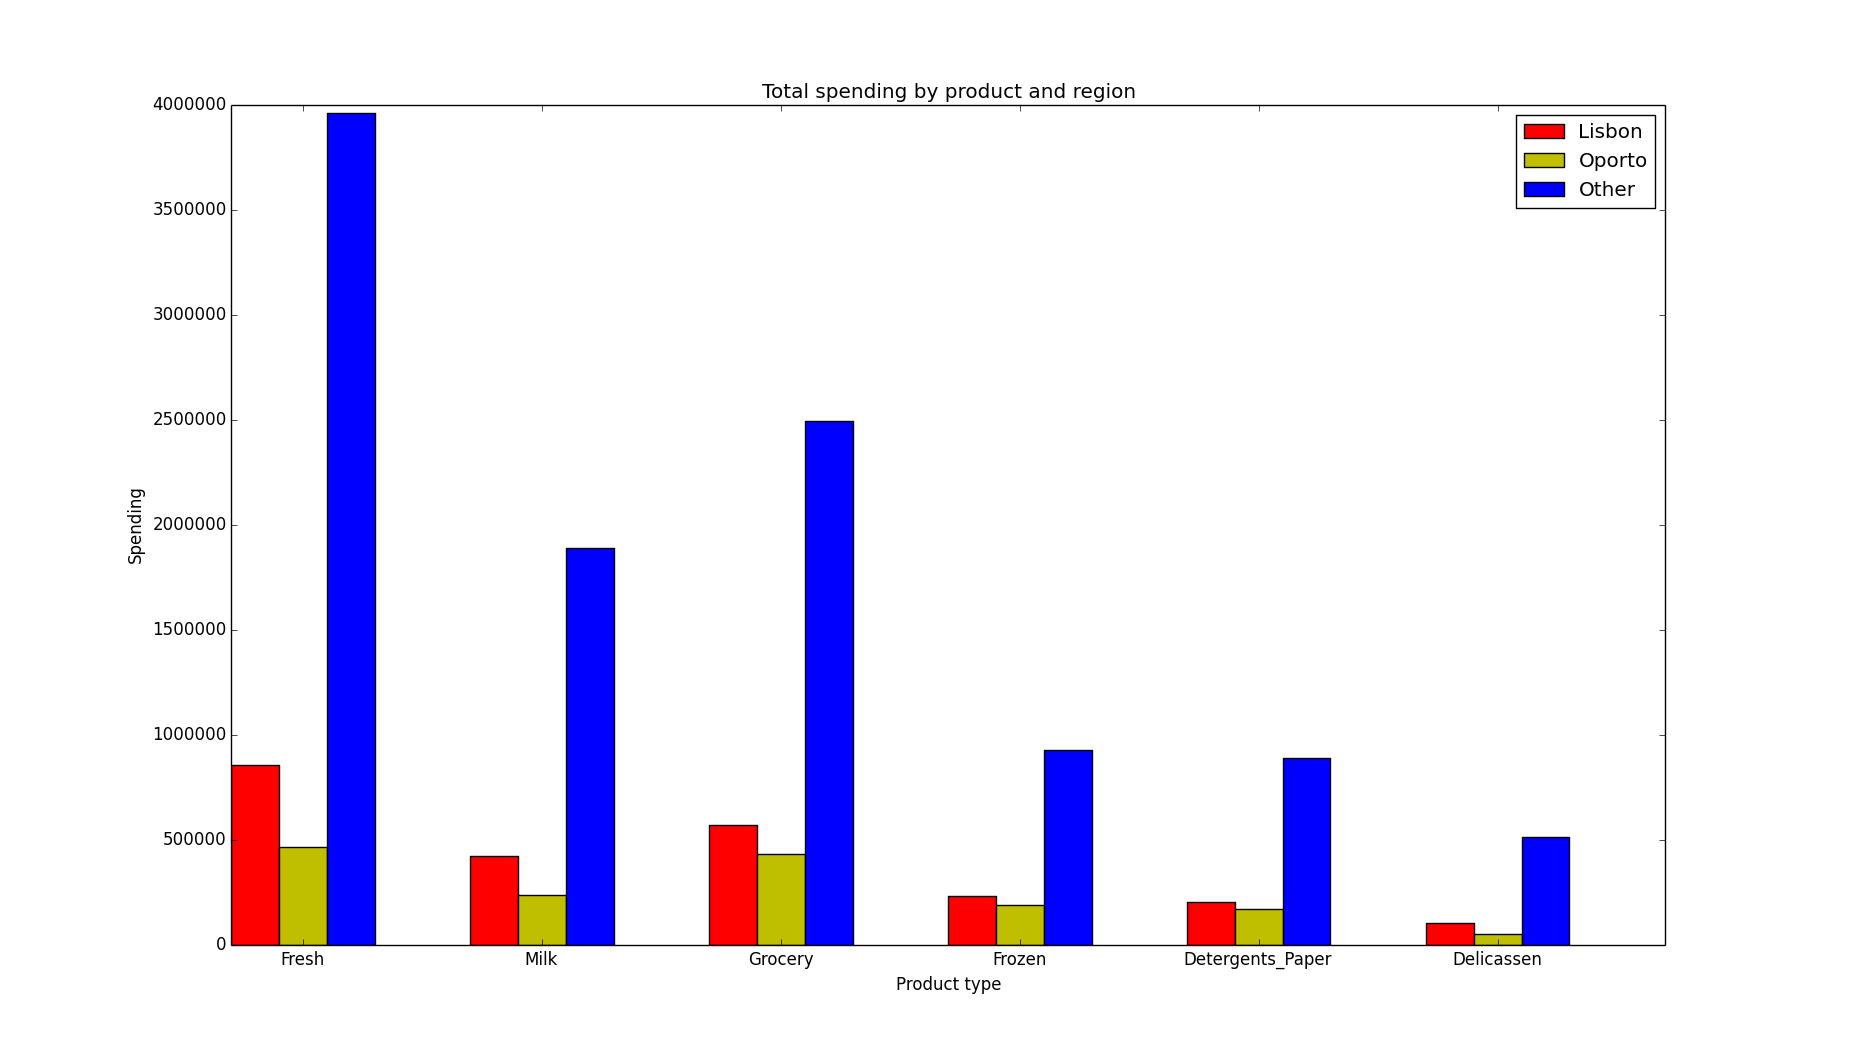
\includegraphics[scale=0.3]{part2a.png}
		\caption{Total spending by region}
	\end{figure}
	\begin{figure}
		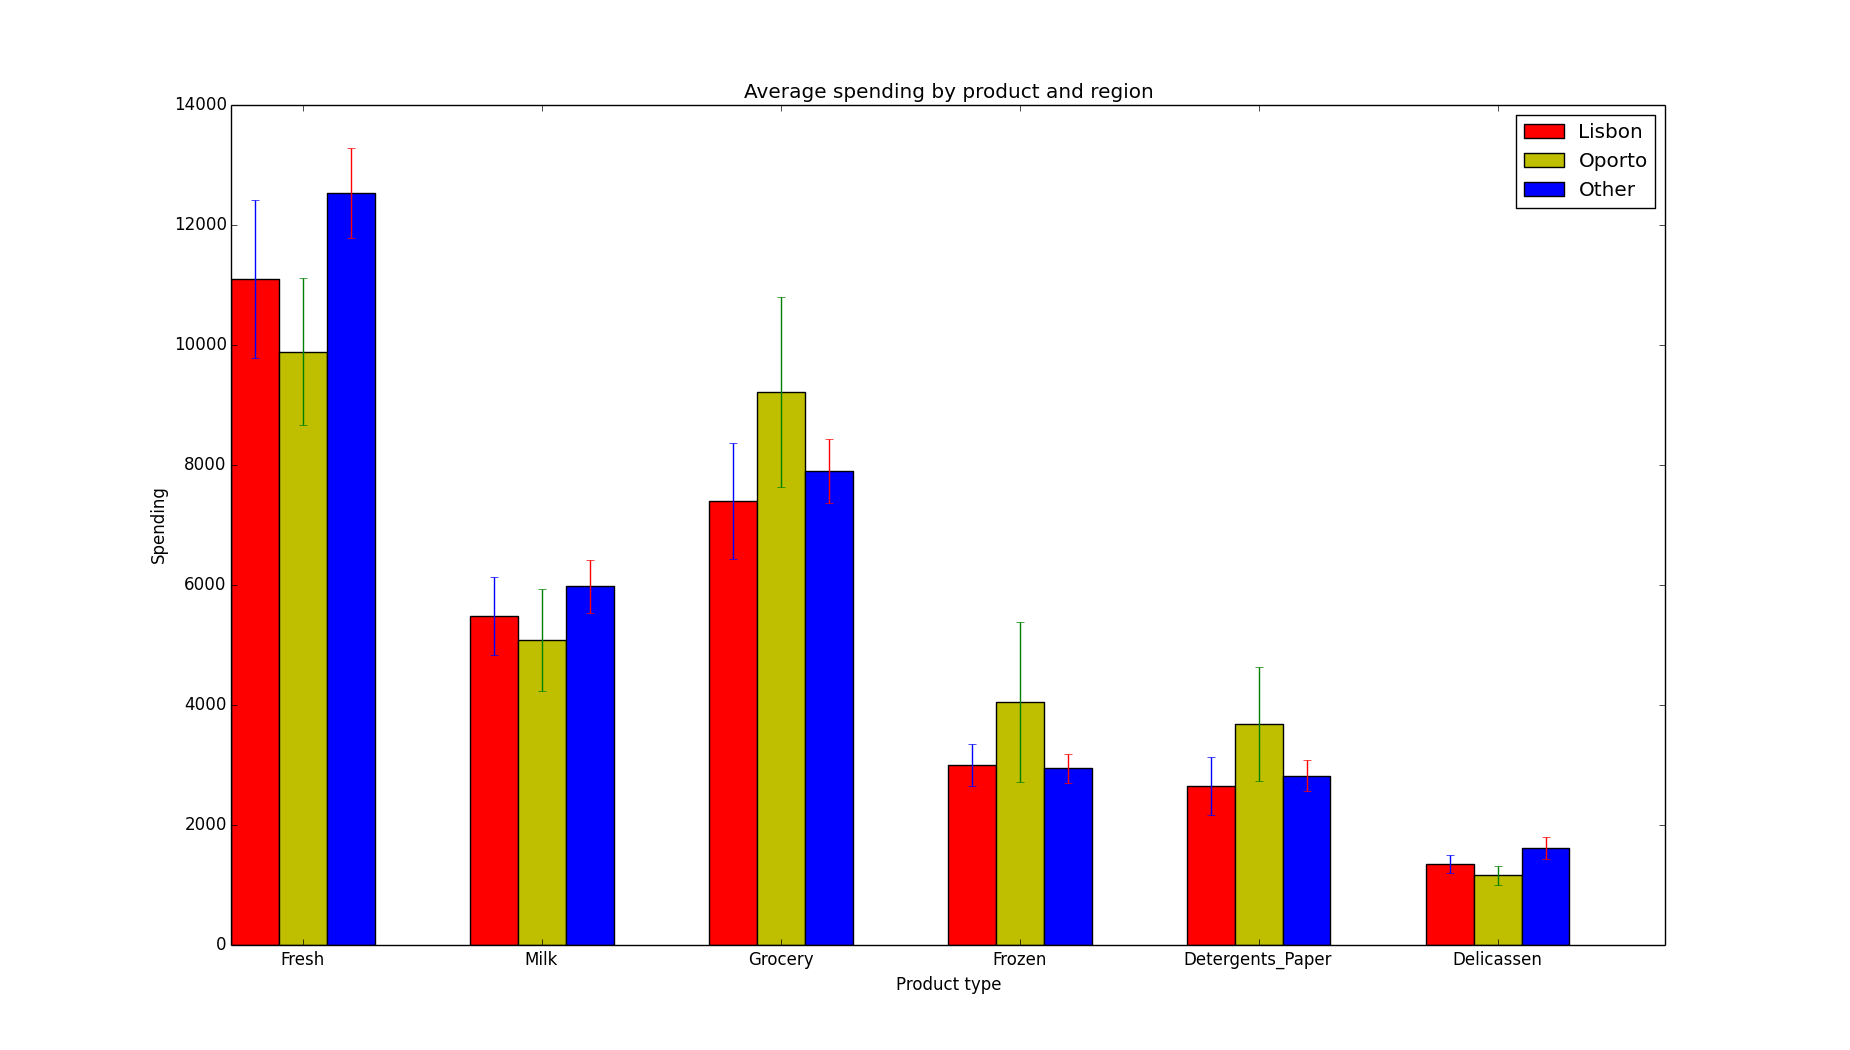
\includegraphics[scale=0.3]{part2b.png}
		\caption{Average spending by region}
	\end{figure}
	
	\newpage
	
	\noindent
	\textbf{Part 3}\\
	\begin{figure}
		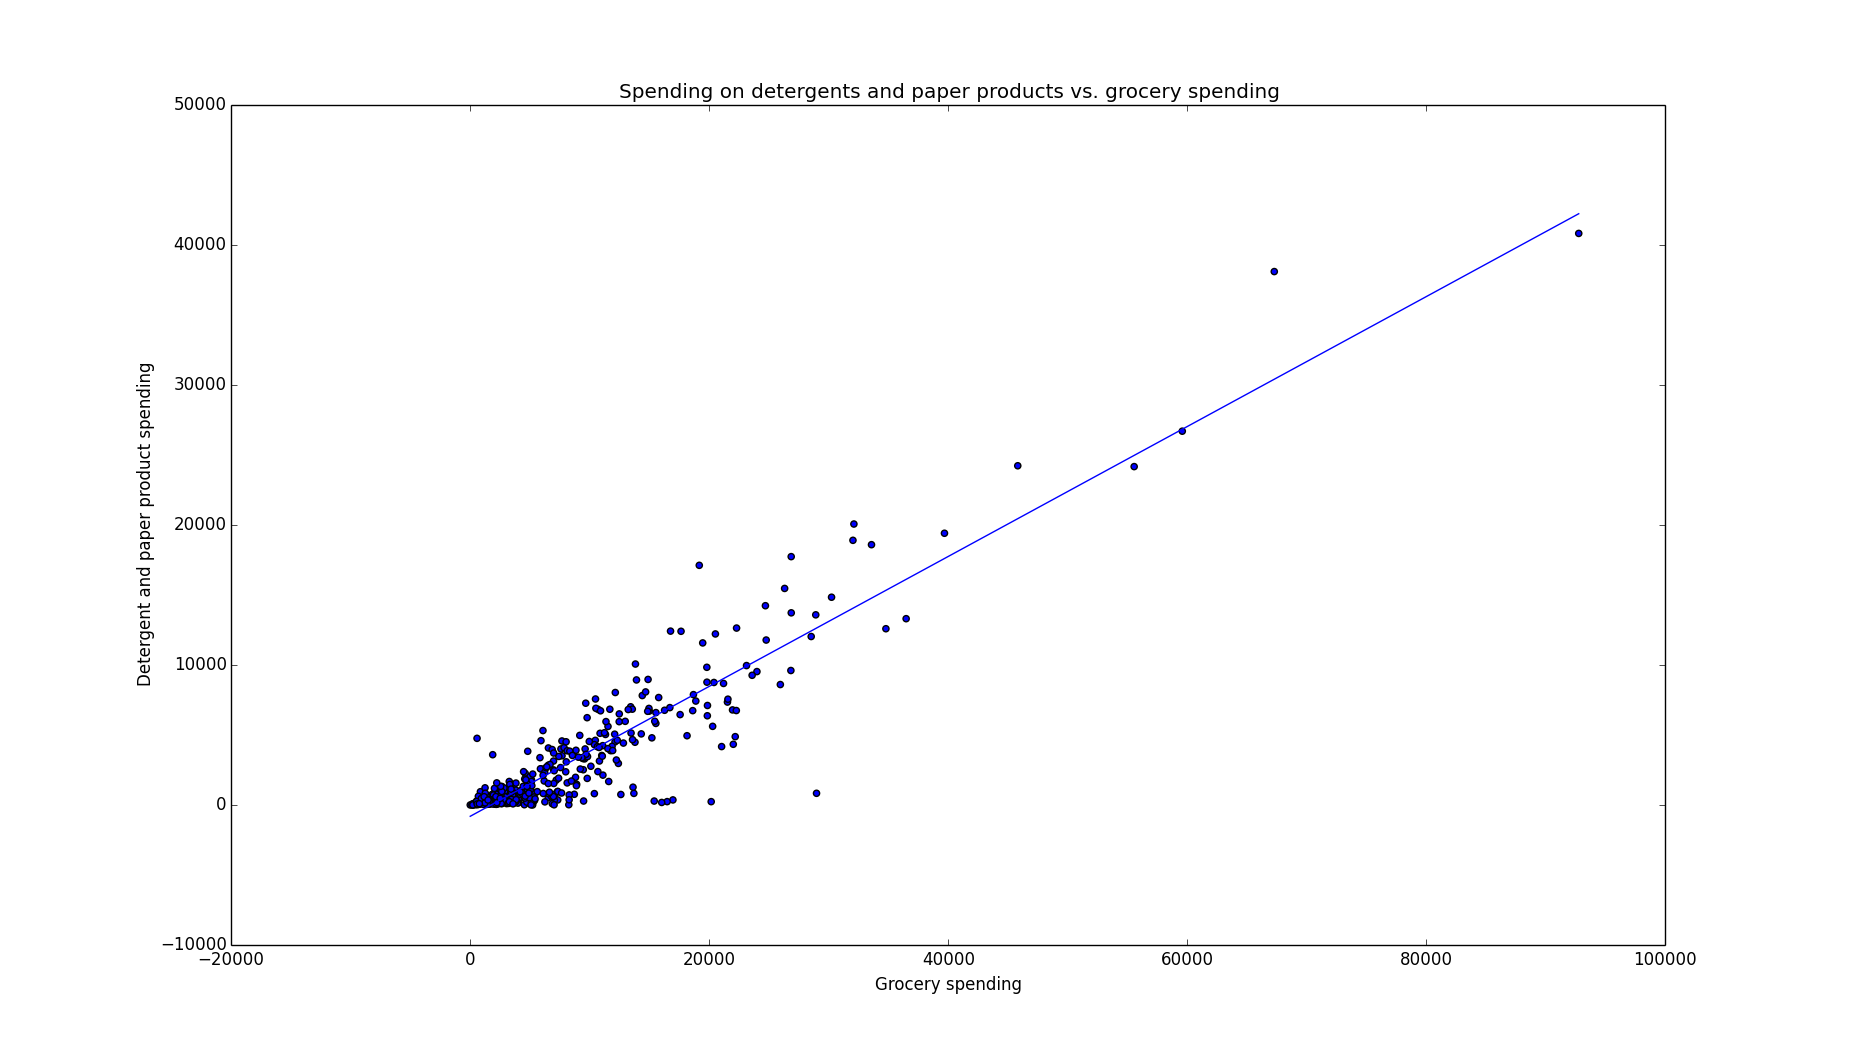
\includegraphics[scale=0.3]{part3.png}
		\caption{Relationship between spending on groceries and spending on detergents and paper, with data and best-fit line}
	\end{figure}
	There is a strong correlation between spending on groceries and spending on detergents and paper. Here is the summary:
	\begin{lstlisting}[basicstyle=\tiny]
                            OLS Regression Results                            
==============================================================================
Dep. Variable:       Detergents_Paper   R-squared:                       0.855
Model:                            OLS   Adj. R-squared:                  0.855
Method:                 Least Squares   F-statistic:                     2582.
Date:                Wed, 14 Sep 2016   Prob (F-statistic):          9.56e-186
Time:                        17:29:39   Log-Likelihood:                -3925.7
No. Observations:                 440   AIC:                             7855.
Df Residuals:                     438   BIC:                             7864.
Df Model:                           1                                         
Covariance Type:            nonrobust                                         
==============================================================================
                 coef    std err          t      P>|t|      [95.0% Conf. Int.]
------------------------------------------------------------------------------
Intercept   -807.1336    113.050     -7.140      0.000     -1029.322  -584.945
Grocery        0.4639      0.009     50.812      0.000         0.446     0.482
==============================================================================
Omnibus:                       97.684   Durbin-Watson:                   1.932
Prob(Omnibus):                  0.000   Jarque-Bera (JB):             1291.839
Skew:                          -0.511   Prob(JB):                    3.02e-281
Kurtosis:                      11.332   Cond. No.                     1.62e+04
==============================================================================
	\end{lstlisting}
	
	\noindent
	\textbf{Part 4}\\
	Below is the code I used to generate the images in parts 2 and 3. See \url{https://github.com/andrew-lei/cse494/blob/master/HW1/hw1.py} for the file.
	
	\begin{lstlisting}[language=python]
#! /usr/bin/env python

import pandas as pd
import matplotlib.pyplot as plt
import numpy as np
import statsmodels.formula.api as sm

# Read the data
data = pd.read_csv('Wholesale customers data.csv')
totals = []
means = []
stderrs = []

# Compute average spending by category
for i in range(1, 4):
    # Get data from region i (1, 2, or 3) for spending on Fresh, Milk, &c.
    regdata = data[data.Region == i][['Fresh', 'Milk', 'Grocery', 'Frozen', 'Detergents_Paper', 'Delicassen']]
    totals += [regdata.sum().as_matrix()]
    means += [regdata.mean().as_matrix()]
    # Compute standard error of mean
    stderrs += [ regdata.std().as_matrix() / np.sqrt(len(regdata)) ]


ind = np.arange(6)  # The x locations for the groups; 0, 1, 2, ..., 5
width = 0.2       # The width of the bars
fig, ax = plt.subplots()
fig.set_size_inches(18.5, 10.5) # Default size is too small

# Bars for bar graph - using total
rects = [ax.bar(ind, totals[0], width, color='r'),
    ax.bar(ind + width, totals[1], width, color='y'),
    ax.bar(ind + 2*width, totals[2], width, color='b')]

# Labels, titles, ticks, &c.
ax.set_xlabel('Product type')
ax.set_ylabel('Spending')
ax.set_title('Total spending by product and region')
ax.set_xticks(ind + 1.5 * width)
ax.set_xticklabels(['Fresh', 'Milk', 'Grocery', 'Frozen', 'Detergents_Paper', 'Delicassen'])
ax.legend((rects[0][0], rects[1][0], rects[2][0]), ('Lisbon', 'Oporto', 'Other'))

# Save and clear for next image
plt.savefig('part2a.png')
plt.cla()

# Bars for bar graph - using mean
rects = [ax.bar(ind, means[0], width, color='r', yerr=stderrs[0]),
    ax.bar(ind + width, means[1], width, color='y', yerr=stderrs[1]),
    ax.bar(ind + 2*width, means[2], width, color='b', yerr=stderrs[2])]

# Labels, titles, ticks, &c.
ax.set_xlabel('Product type')
ax.set_ylabel('Spending')
ax.set_title('Average spending by product and region')
ax.set_xticks(ind + 1.5 * width)
ax.set_xticklabels(['Fresh', 'Milk', 'Grocery', 'Frozen', 'Detergents_Paper', 'Delicassen'])
ax.legend((rects[0][0], rects[1][0], rects[2][0]), ('Lisbon', 'Oporto', 'Other'))

# Save and clear for part 3
plt.savefig('part2b.png')
plt.cla()

# Ordinary least squares fit for Grocery (independent) and Detergents_Paper(dependent)
fit = sm.ols(formula="Detergents_Paper ~ Grocery", data=data).fit()
ind = np.arange(min(data['Grocery']), max(data['Grocery']) )

print fit.summary()
print fit.pvalues # Print separately because very close to zero

# Plot points and best-fit
ax.scatter(data['Grocery'], data['Detergents_Paper'])
ax.plot(ind, fit.params[0] + ind*fit.params[1])

# Labels and title
ax.set_xlabel('Grocery spending')
ax.set_ylabel('Detergent and paper product spending')
ax.set_title('Spending on detergents and paper products vs. grocery spending')

# Save
plt.savefig('part3.png')
	\end{lstlisting}
	
\end{document}